A continuación definimos formalmente el problema composicional de síntesis de controlador nonblocking.

\begin{definition}[Autómata Determinístico] \label{def:automata}
	Un \k{autómata determinístico} es una tupla $T = (S_T, A_T, \D_T, \init{t}, M_T)$, donde:
	\begin{itemize*}[label=]
		
		\item $S_T$ es un \k{conjunto finito de estados};
		
		\item $A_T$ es el \k{conjunto de eventos} del autómata;
		
		\item $\D_T \C (S_T \x A_T \x S_T)$ es una \k{función de transición};
		
		\item $\init{t} \in S_T$ es el \k{estado inicial}; y
		
		\item $M_T \C S_T$ es un conjunto de \k{estados marcados}.
		
	\end{itemize*}
	
\end{definition}

\begin{notation}[Pasos y corridas] \label{not:paso}
	
	$\!\!$Notamos $(t,\l,t') {\in}\!\! \D_T$ como $t \step{\l}{T} t'$ y lo llamamos \k{paso}.
	A su vez, una \k{corrida} de una palabra $w = \l_0,\ldots,\l_k$ en $T$, es una secuencia de pasos tal que $t_i \step{\l_i}{T} t_{i+1}$ para todo $0 \leq i \leq k$, notado como $t_0 \runw{w}{T} t_{k+1}$.
	
\end{notation}

Los autómatas definen un lenguaje, un conjunto de palabras, que aceptan. Dado un conjunto de eventos $A$, notamos con $A^*$ al conjunto de palabras finitas de eventos de $A$. El lenguaje generado por un autómata $T$ es el conjunto de palabras formadas por sus eventos que cumplen $\D_T$. Formalmente, si $w \in A_T^*$, entonces $w \in \L(T)$ si y solo si existe una corrida para $w$ comenzando desde el estado inicial $\init{t}$ de $T$, que notamos $\init{t} \runw{w}{T} t_{k+1}$.


\begin{definition} [Composición Paralela] \label{def:parcomp}
	La \k{composición paralela} $(\|)$ de dos autómatas $T$ y $Q$ es un operador simétrico y asociativo que produce un autómata $T \| Q = (S_T {\times} S_Q, A_T {\cup} 
	A_Q, \D_{T\|Q}, \<\init{t},\init{q}\>, M_T {\times} M_Q)$, donde $\D_{T\|Q}$ es la menor relación que satisface las siguientes reglas (omitimos la versión simétrica de la primera regla):
	
	\begin{normalsize}
		\centering
		\vspace{-18pt}
		\hspace{-50pt}
		\begin{minipage}{0.30\linewidth}
			\[ 
			\frac{t \step{\l}{T} t'}{\<t,q\> {\step{\l}{T\|Q}} \<t'\!,\!q\> }{{\scriptstyle \l \in A_{T} {\setminus} A_{Q}}} 
			\]
		\end{minipage} 
		\hspace{40pt}
		%\begin{minipage}{0.30\linewidth}
		%\[ 
		%\frac{q \step{\l}{Q} q'}{\<t,q\> \step{\l}{T\|Q} \<t,q'\>}{{\scriptstyle \l \in A_{\!Q} 
		%{\setminus} A_{T}}} 
		%\]
		%\end{minipage} \\[-6pt]
		%\hspace{-20pt}
		\begin{minipage}{0.30\linewidth}
			\[ 
			\frac{t \step{\l}{T} t' \quad q \step{\l}{Q} q'}{\<t,q\> \step{\l}{T\|Q} \<t',q'\>}{{\scriptstyle \l \in A_{T} {\cap} A_{Q}}}
			\]
		\end{minipage} \\[15pt]
	\end{normalsize}
\end{definition}

\section{Controlador objetivo}

Dado un autómata y una partición de sus eventos en dos subconjuntos: $controlables$ y $no controlables$, lo que buscamos es un $controlador$ (director) que restrinja el vocabulario aceptado de forma de mantener un camino posible a los estados marcados del autómata.

Un controlador observa las transiciones no controlables y deshabilita alguna transiciones controlables para generar una planta restringida. Una palabra $w$ pertenece al lenguaje generado por $T$ restringido por una función del controlador $\sigma : A_T^* \into 2^{A_T}$ (anotado como $\L^\sigma(T)$) si cada prefijo de $w$ ``sobrevive'' a $\sigma$.
Formalmente, sea $w = \l_0,\ldots,\l_k$ una palabra en $\L(T)$, entonces $w \in \L^\sigma(T)$ si y solo si para todo $0 \leq i \leq k$:
$
\init{t} \run{\,\l_0}{\l_i}{T} t_{i+1} \wedge \l_i \in \sigma(\l_0,\ldots,\l_{i-1})
$

\begin{definition}[Problema de Control Safe y Non-Blocking] \label{def:control-problem}
	Un \k{Problema de Control} con objetivos \k{Safe} y \k{Non-Blocking} composicional es una tupla $\E = (E, A_E^C)$, donde $E$ es un conjunto de autómatas $\{E_0,\ldots,E_n\}$ (podemos abusar la notación y usar $E = (S_E,A_E,\D_E,\init{e},M_E)$ para referirnos a la composición $E_0\|\ldots\|E_n$), y $A_E^C \C A_E$ es el conjunto de eventos controlables (i.e., $A_E^U = A_E \setminus A_E^C$ es el conjunto de eventos no controlables).
	Una solución para $\E$ es un supervisor $\sigma : A_E^* \into 2^{A_E}$, tal que $\sigma$ es:
	\begin{itemize}[itemsep=4pt,topsep=-8pt]
		
		\item \k{Controlable}: $A_E^U \C \sigma(w)$ con $w \in A_E^*$; y
		
		\item \k{Safe y Nonblocking}: para cada palabra $w \in \L^\sigma(E)$ existe una palabra no vacía $w' \in A_E^*$ tal que, la concatenación $ww' \in \L^\sigma(E)$ y $\init{e} \runw{\;ww'}{E} e_m$ con $e_m \in M_E$ (i.e., un estado marcado de $E$).
		
	\end{itemize}
	
\end{definition}

Podemos pensar en un controlador non-blocking como un jugador optimista. Se encarga de no perder, y mientras tenga un futuro camino posible que lo lleva al destino buscado, considera que está ganando.

Es clave entender que en el problema a tratar, la posición de "tablas" del ajedrez, en la que ambos jugadores repiten sus jugadas 50 veces, se considera ganadora si todavía hay opción de dar un jaque mate. Si repetimos nuestras jugadas y todavía tengo dos torres considero que gané el partido, porque eventualmente mi oponente podría cansarse y dejarme ganar. Si repetimos nuestras jugadas pero solo tengo mi rey, no hay forma de dar mate, no puedo extender esta "palabra", esta partida, de forma de dar mate, y considero que perdí.

Es importante notar que como se busca que cualquier palabra sea extendible a otro estado marcado, lo que se busca es pasar por algún estado marcado infinitas veces. O sea, un estado 'e' marcado que tenga un camino para que el jugador pueda volver controlablemente al mismo estado 'e'.

Por esto, las estructuras claves que analizamos en nuestro algoritmo son los ciclos ($loops$), ya que los primeros estados ganadores son aquellos que están en un loop controlable con un estado marcado dentro. Luego anotamos como ganadores también a cualquier estado que controlablemente alcanza un estado ganador.

Los ciclos también son esenciales para encontrar los estados perdedores, ya que la única forma de que un estado sea perdedor es que no pueda alcanzar un estado ganador. En otras palabras, los estados perdedores son aquellos que forman parte de un loop que no tiene estados marcados ni transiciones salientes.

De forma más concreta, en nuestro algoritmo, un ciclo del cual el jugador no puede escapar, pero desde el cual existe un camino hacia un estado ganador, se considera ganador.

\section{Director} \label{chpt:director}
En particular, buscamos como solución al problema de control, controladores que sean directores, como en \textcolor{red}{[REFS Huang]}. Un director se destaca por habilitar a lo sumo un evento controlable en cada punto de la ejecución. 

\begin{definition}[Director] \label{def:director}
	Dado un controlador $\sigma : A_E^* \into 2^{A_E}$ de un problema de control $\E$, decimos que $\sigma$ es un director si $\forall w \in A_E^*$, $\|\sigma(w) \cap A_E^C\| \leq 1$.	
\end{definition}

Esto es en contraste con las soluciones tradicionales de Discrete Event Control y sus herramientas, como \textcolor{red}{poner a SUP?} que presentan supervisores maximales. Los supervisores deben habilitar todos los eventos controlables que sean válidos en algún controlador que cumpla el objetivo del problema. Es decir que un director será un controlador que cumpla el mismo objetivo que un supervisor, pero restringiendo las palabras posibles a un subconjunto del lenguaje aceptado por el supervisor.

El foco en la construcción de directores tiene las siguientes razones:

\begin{itemize}
	\item Los directores pueden ser más apropiados en contextos donde el controlador \textit{ejecuta} las acciones controlables \textcolor{red}{REF}.
	
	\item La construcción de directores puede requerir una menor exploración de la planta que la construcción de un supervisor. Esto se sinergiza y potencia las ganancias en tiempo de la técnica al explorar la composición on-the-fly y permite componer una proporción menor de la planta.
	
	\item En el caso de poder sintetizar un director explorando menos de la planta, se podría usar tanto para controlar la planta como para probar la controlabilidad de un problema donde herramientas de construcción de supervisores fallan por tener que explorar en mayor medida un problema de gran tamaño.
	
	\item Hay hasta la fecha una falta de herramientas disponibles para la síntesis de directores
\end{itemize}

Notar que en \textcolor{red}{[REF 15 paper]} se prueba que un director existe si y solo si un supervisor maximal existe.

\section{Algoritmo monolítico} \label{chpt:algoMono}

Una solución a este problema, anteriormente estudiada~\cite{Ehlers:EECS-2013-162} se basa en un menor punto fijo. Simplemente se comienza con el conjunto de los estados que no tienen ningún camino para alcanzar un estado marcado. Luego en cada iteración se agrega al conjunto de los estados perdedores todos aquellos que en un paso son forzados al conjunto de la iteración anterior. 

Si al concluir el punto fijo el estado inicial no se encuentra en el conjunto entonces existe un controlador para el problema en cuestión y para construirlo se deben evitar las transiciones controlables que llevan al conjunto de estados perdedores.

Presentamos en el listing~\ref{lst:classical} una simplificación del algoritmo monólitico (que resuelve toda la planta ya compuesta).

\begin{lstlisting}[language={pseudocode},label={lst:classical},caption={Algoritmo Monolitico},float=ht]
Algorithm classicalSolver($E, A_E^C$):
	$B = \{s \in S_E \mid \nexists w \ldot \trimlst{s \runw{w}{E} m} \wedge m \in M_E \}$
	$B' = \emptyset$
	while $B' \neq  B:$
		$B' = B$
		$B = B \cup \{s \in S_E \mid $forcedTo($s,e,E$)$\wedge e \in B \}$
	return $\initial \notin B$
\end{lstlisting}

Nuestro problema surge de que para el primer paso, encontrar el conjunto $B$ inicial de estados que no alcanzan un marcado, necesitaríamos conocer los caminos que puede tomar cualquier estado, lo cual implica componer toda la planta.

Sin embargo, utilizamos la idea del punto fijo que detecta errores en la función \texttt{findNewGoalsIn} ya que en ese momento no lo podemos evitar, y simplemente asumimos que lo no explorado no puede llegar a un estado marcado. Esto se discutirá en mayor profundidad en el capítulo~\ref{chpt:dcs}.

\section{Exploración on-the-fly}

El problema de síntesis de controlador ya tiene una solución clásica, por lo que la dificultad del trabajo no consistió en desarrollar un algoritmo que detectara estados ganadores y perdedores de un LTS totalmente explorado. 

El conflicto reside en que al componer distintos DES, la cantidad de estados de la composición es exponencial respecto de los estados en los componentes. Esto es de suma relevancia ya que la solución clásica, que compone toda la planta para luego explorarla, tiene un límite de escalabilidad en el cual la composición de la planta llega al límite de tiempo o memoria, y nunca se llega a la exploración.

Para combatir esto, la exploración on-the-fly clasifica estados como ganadores o perdedores durante la composición. Se espera que con esto sea posible, en primer lugar, cortar la exploración de una rama de la planta que ya se sabe que es perdedora o ganadora, reduciendo así la memoria y tiempo necesarios. Pero más aún, si el estado inicial fuera marcado como ganador o perdedor antes de la composición completa de la planta, ni siquiera sería necesario completar el proceso de composición.

En el listing \ref{lst:on-the-fly} mostramos la estructura básica de este método. Consiste en ir agregando una transición a la vez a la parte conocida de la planta, y en cada paso ver si esta nueva transición permite concluir que un estado es ganador o perdedor. Si algún nuevo estado se clasifica como ganador  o perdedor, se propaga esta información a sus antecesores, posiblemente marcándolos a su vez como perdedores o ganadores.

\begin{lstlisting}[language={pseudocode},label={lst:on-the-fly},caption={Algoritmo Monolitico},float=ht]
Algorithm genericOTF-Exploration($E, A_E^C$):
   $\initial$ = $\<\init{e}^0,\ldots,\init{e}^n\>$
   $\structure = initial$ //la parte conocida de la planta
   while $initial \notin \Goals \cup \Errors$:
     $(e,\l,e') = $proxTransicion($\structure$)
     expandirES($\structure,(e,\l,e')$)
     if $e' \in \Errors$:
       propagarError($e'$)
     else if $e' \in \Goals$:
       propagarGoal($e'$)
     else if isLoop($e,e'$):
       if nuevoLoopGanador($e,e'$):
         propagarGoal($e'$)
       else if nuevoLoopPerdedor($e,e'$):
         propagarError($e'$)
         
   if $initial \in \Goals$:
     return armarControlador($\Goals$)
   else:
     return "UNREALIZABLE"  
\end{lstlisting}

Para incrementar las ramas podadas se utiliza una heurística de exploración Best First Search \cite{tesisDani} que busca ganar controlablemente o perder no controlablemente, para garantizar con la menor exploración posible que el estado actual es ganador o perdedor.

En el peor caso, no se pudo concluir nada antes de componer la planta en su totalidad, se perdió tiempo en los puntos fijos, intentando clasificar estados, y se realiza una última vez el algoritmo clásico con la planta totalmente explorada. Esto garantiza la completitud del algoritmo, como se detalla en mayor profundidad en el capítulo~\ref{chpt:dcs}.

En todos los gráficos siguientes vamos a utilizar las letras $c$, $u$, para denotar si una transición es controlable o no, respectivamente; en caso de no especificar letra para una transición es porque su controlabilidad no afecta el resultado del ejemplo.

\subsection{marcado explícito errores}

Gracias a esta suite de tests pudimos encontrar que la exploración fallaba en tres puntos importantes:
\begin{itemize}
	\item Falencias al encontrar errores
	\item Propagación local
	\item Falta de completitud en la exploración en casos donde era necesario seguir.
	\item detección de estados ganadores poco robusta.
\end{itemize}

% FALENCIAS AL ENCONTRAR ERRORES
En cuanto a agregar estados al conjunto $\Errors$ la inadvertencia se debía a que no sacaba conclusión alguna al haber explorado todo un sub-autómata, por ende al propagar información desde otra rama se podría llegar a un resultado erróneo. 

Para comprender mejor observar la figura \ref{fig:falenciasErrores} donde desde el estado e tenemos dos sub-ramas a explorar. Si se mira primero la rama de abajo y no lo marcamos como error, a pesar de estar completamente explorado, entonces al mirar la de arriba diremos que es goal y propagaremos dicha información, equivocadamente, más allá de e. 

Cabe destacar que esto era posible debido a que no se requería que un estado hijo tenga conclusión\footnote{Es decir, esté en el conjunto $\Goals$ o $\Errors$} para seguir propagando, es decir, bastaba con que haya sido explorado alguna vez y se asumía lo mejor.
\begin{figure}[htb]
	\centering
	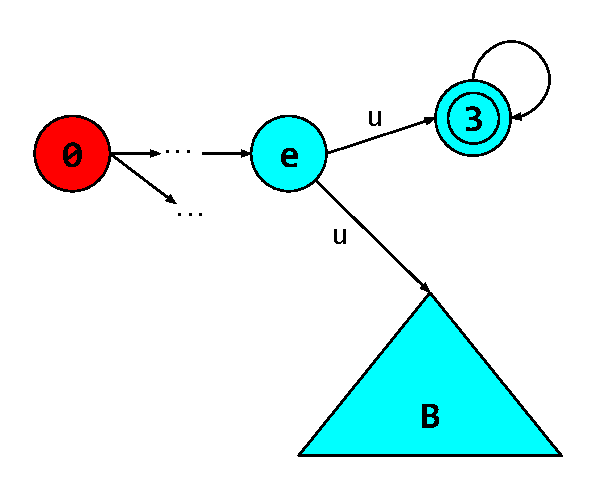
\includegraphics[width=\linewidth/2]{figures/FalenciasErrores.pdf}
	\caption{Caso no controlable que anteriormente propagaba Goal}
	\label{fig:falenciasErrores}
\end{figure}

\subsection{Propagación local vs por conjuntos}

% PROPAGACION LOCAL
Por otro lado, al propagar tenía una mirada local, perdiendo información sobre lo que sucede dentro del conjunto. Es así que no podía reconocer casos donde, por ejemplo: hay un loop controlable entre dos estados, el cual se explora primero, y uno de ellos va controlablemente a un error. En este caso es obvio que todo debe ser error pero según la mirada local ambos tienen \textit{una forma de escapar del error}, el otro estado del conjunto. Para una aclaración visual ver la fugura \ref{fig:propagarError}.

Equivalentemente tampoco funciona reconociendo $\Goals$, en la figura \ref{fig:propagarGoal} se puede ver un ejemplo. El estado $2$ llega al estado marcado $3$, pero no puede forzarlo. Por ser non-blocking esto no nos molestaría y el modelo debería ser controlable. Pero si miramos localmente al propagar $Goal$ desde $3$, no sabemos dónde nos lleva la transición no controlable, y deberíamos suponer lo peor.

En conclusión, es difícil decidir dónde hacer el corte. Son muchos casos y no se puede, localmente, distinguirlos a todos. Por ende es necesario un algoritmo más inteligente, con una mirada global del conjunto a propagar.
\begin{figure}[htb]
	\centering
	\makebox[\linewidth][c]{%
		\begin{subfigure}[t]{.5\textwidth}
			\centering
			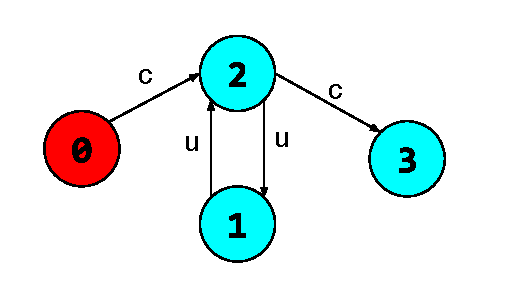
\includegraphics[width=\linewidth]{figures/PropagarError.pdf}  
			\caption{Propagar errores}
			\label{fig:propagarError}
		\end{subfigure}
		\begin{subfigure}[t]{.5\textwidth}
			\centering
			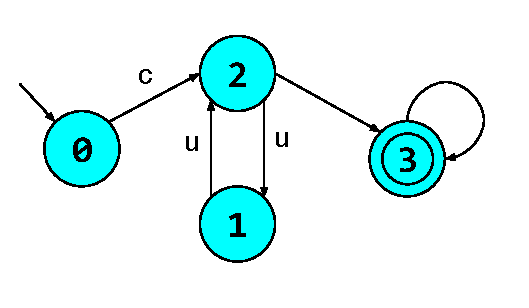
\includegraphics[width=\linewidth]{figures/PropagarGoal.pdf}  
			\caption{Propagar goals}
			\label{fig:propagarGoal}
		\end{subfigure}
	}
	\caption{Problemas de propagación local.}
	\label{fig:propagacionLocal}
\end{figure}

\subsection{Completitud de exploración}

% FALTA DE COMPLETITUD
Respecto a la falta de completitud, queda claro que teniendo una conclusión para cada uno de los estados hijos del inicial podemos definir si el problema es o no controlable. 
Lo que sucedía era que al tener conclusiones erróneas y problemas de propagación había ciertos casos donde, según el algoritmo de exploración el problema era controlable pero al llegar al constructor del controlador se daba cuenta que había estados a los cuales les faltaba exploración y que, de hecho, tenían transiciones no controlables a estados sin mirar. 
Llegado ese punto devolvía que no había controlador, cuando de seguir explorando hubiese visto que lo que faltaba era algo ganador. Un ejemplo particular de esto puede verse en la figura \ref{fig:faltaCompletitud}, al terminar la exploración se concluyó que era controlable, sin embargo al querer construir el controlador se descubre que el estado $1$ tiene una no controlable por explorar, devolviendo entonces que no existe controlador. 

\begin{figure}[htb]
	\centering
	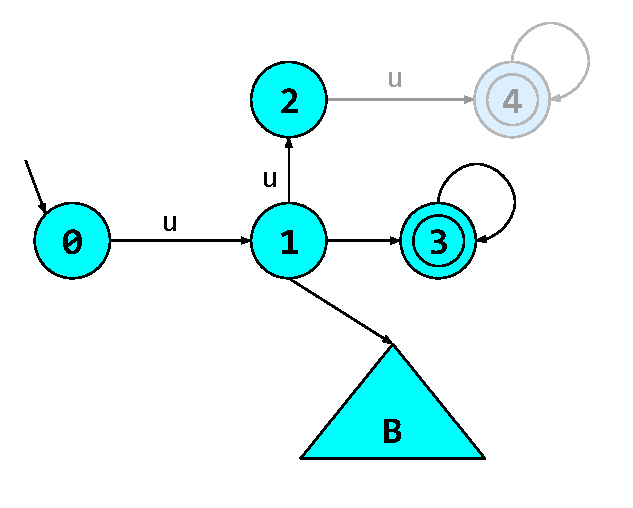
\includegraphics[width=\linewidth/2]{figures/faltaDeCompletitud.pdf}
	\caption{Ejemplo de falta de completitud, los estados en gris son los faltantes por explorar.}
	\label{fig:faltaCompletitud}
\end{figure}

\subsection{Correcta detección de loops ganadores}

La detección de loops con estados ganadores es una pieza central del problema, y tampoco puede solucionarse con una mirada local. Originalmente, la primera versión del pseudocódigo daba una descripción declarativa de los estados a encontrar (ver listng \ref{lst:viejoMCCC}). Esta descripción de los estados en un loop ganador es correcta, pero no resulta claro como implementarla. En particular, fue claro al incrementar la batería de tests que la detección de loops ganadores necesitaba una modificación.

Luego de varias intentos más veloces (como ejemplo ver el pseudocódigo de \texttt{findNewErrorsIn($loops$)}) pero que presentaban fallas, llegamos a la conclusión de utilizar un algoritmo de punto fijo clásico (similar a listing \ref{lst:classical}) pero con una planta reducida. Como se verá más adelante, corremos el algoritmo clásico sobre una versión optimista que asume que toda transición no explorada es perdedora, y de los estados ya explorados solo tomamos en cuenta un grupo reducido que forma un loop sobre la última transición explorada. Este enfoque otorga la completitud del algoritmo tradicional mientras que sostiene la eficiencia de la exploración on-the-fly.

\begin{lstlisting}[language={pseudocode},label={lst:viejoMCCC},caption={vieja descripción estados ganadores},float=ht, frame=single]
function buildMCCC($e, e'$):
let $C$ such that
$C = \{ e_i \mid (e' \runw{w}{\structure} e_i \runw{w'}{\structure} e \vee e \runw{w}{\structure} e_i \runw{w'}{\structure} e') \wedge $extendsCCC($e_i,C \cup \Goals$)$ \wedge$
$(\exists w \ldot e \runw{w}{\structure} e_m \wedge e_m \in M_E \cap (C \cup \Goals)) \}$
return $C$

function extendsCCC($e, C$):
return $(\exists \l \ldot e \step{\l}{E} e' \wedge e' \in C) \wedge (\forall \l_u \in A_U \ldot e \step{\l_u}{E} e' \Rightarrow e' \in C)$

\end{lstlisting}

\subsection{Agnosticismo a la heurística}

Una distinción clave del algoritmo \textit{on-the-fly} es que está dividido en dos partes. Por un lado se tiene el algoritmo de exploración responsable de que al final se llegue al resultado correcto, por el otro tenemos una heurística que le brinda la próxima transición a explorar. Ese algoritmo de exploración no puede depender de la heurística, ya que la misma, por su nombre, no garantiza siempre elegir el mejor camino posible, sino solo la mejor aproximación que encuentre. Es en esa correctitud independiente de la heurística donde nuestro trabajo hizo foco.

El proyecto \texttt{MTSA} inicialmente contaba con dos heurísticas \texttt{BFS} para exploración, \textit{Monotonic Abstraction} y \textit{Ready Abstraction}. Ambas cumplen su función en síntesis de controlador con exploración parcial, pero presentaban un problema.

El algoritmo de exploración había sido desarrollado en conjunto con las heurísticas y si bien esto ayudaba a la eficiencia del mismo, no resultaba agnóstico a las mismas. El nuevo enfoque no depende de la forma de explorar, por ende, da una mayor libertad de investigar a futuro nuevos criterios de evaluación para mejorar la eficiencia de la técnica sin comprometer correctitud ni completitud.







